%!TEX program = xelatex
\documentclass[8pt, landscape, a4paper]{extarticle}

% --- 核心宏包 ---
\usepackage[UTF8, fontset=fandol]{ctex}
\usepackage[margin=0.8cm, top=1cm, bottom=1.3cm]{geometry}
\usepackage{multicol}
\usepackage{xcolor}
\usepackage{tcolorbox}
\usepackage{enumitem}
\usepackage{amsmath}
\usepackage{amssymb}
\usepackage{fontspec}
\usepackage{tikz}
\usetikzlibrary{arrows.meta, shapes}

% --- 去掉页码 ---
\pagestyle{empty}

% --- 颜色定义 (Gray/Silver 主题) ---
\definecolor{headerblue}{RGB}{96, 125, 139}    % Blue Grey
\definecolor{navcolor}{RGB}{211, 84, 0}        % 导航橙
\definecolor{intuitioncolor}{RGB}{41, 128, 185}% 直觉蓝
\definecolor{accentcolor}{RGB}{192, 57, 43}    % 强调红
\definecolor{section2}{RGB}{22, 160, 133}      % 绿色
\definecolor{dividergray}{RGB}{220, 220, 220}

% --- 全局设置 ---
\setlength{\parindent}{0pt}
\setlength{\columnsep}{0.4cm} 
\linespread{1.1} 

% --- 列表样式 ---
\setlist[itemize]{leftmargin=1.2em, nosep, itemsep=2pt, topsep=2pt, label=$\textcolor{headerblue}{\vcenter{\hbox{\tiny$\bullet$}}}$ }
\setlist[description]{leftmargin=0.2em, style=sameline, nosep, itemsep=2pt, font=\bfseries}

% --- Box 样式 ---
\newtcolorbox{mybox}[2][]{%
  colback=white,
  colframe=#2,
  coltitle=white,
  boxrule=1pt,             
  arc=2mm,                 
  left=4pt, right=4pt, top=3pt, bottom=3pt, 
  toptitle=3pt, bottomtitle=3pt, 
  fonttitle=\bfseries\sffamily\large,
  title={#1},
  after skip=5pt          
}

% --- 自定义命令 ---
\newcommand{\subt}[1]{{\vspace{2pt}\textbf{\large \textcolor{black}{#1}}}}

\newcommand{\boxdesc}[1]{%
    \textit{\small \textcolor{gray}{#1}}%
    \par\vspace{2pt}%
    {\color{dividergray}\hrule height 0.5pt}%
    \vspace{2pt}%
}

\newcommand{\sepline}{%
    \par \vspace{3pt}%
    {\color{dividergray}\hrule height 0.5pt}%
    \par \vspace{3pt}%
}

% 公式间距
\setlength{\abovedisplayskip}{3pt}
\setlength{\belowdisplayskip}{3pt}

\begin{document}

% --- 页眉 ---
\begin{center}
    {\Huge \textbf{\sffamily \textcolor{headerblue}{数值分析 Numerical Analysis Cheat Sheet}}} \\
    \vspace{0.2cm}
    {\large \texttt{The Art of Approximation: Solving the Unsolvable}}
\end{center}

% --- 开始四栏布局 ---
\begin{multicols*}{4}

% === 第一栏 ===

\begin{mybox}[️ 场景导航 (Use Cases)]{navcolor}
    \boxdesc{遇到什么问题 $\to$ 用什么工具}
    \begin{itemize}[itemsep=2pt]
        \item \textbf{解非线性方程} $\to$ 牛顿法 (Newton's)
        \item \textbf{解大型线性方程组} $\to$ 迭代法 (GMRES / CG)
        \item \textbf{函数拟合/插值} $\to$ 样条插值 (Spline)
        \item \textbf{数值积分} $\to$ 高斯求积 (Gaussian Quad)
        \item \textbf{解微分方程} $\to$ 龙格-库塔 (Runge-Kutta)
        \item \textbf{特征值计算} $\to$ 幂法 / QR 算法
    \end{itemize}
\end{mybox}

\begin{mybox}[1. 误差与浮点数 (Errors)]{headerblue}
    \boxdesc{计算机不是数学家}
    
    \subt{IEEE 754 浮点数}
    $$ x = (-1)^s \times (1.m) \times 2^{e-127} $$
    \begin{itemize}
        \item \textbf{机器精度 ($\epsilon$)}: $1+\epsilon \neq 1$ 的最小正数 ($\approx 10^{-16}$ for double)。
        \item \textbf{大数吃小数}: $10^{16} + 1 = 10^{16}$。
    \end{itemize}
    \sepline
    
    \subt{稳定性 (Stability)}
    算法对输入微小扰动的敏感度。
    \textbf{条件数}: $\kappa = \frac{|\delta \text{Output}|}{|\delta \text{Input}|}$。
\end{mybox}

\begin{mybox}[2. 根查找 (Root Finding)]{headerblue}
    \boxdesc{求 $f(x)=0$}
    
    \subt{二分法 (Bisection)}
    区间减半。绝对收敛,但慢 (线性)。
    \sepline
    
    \subt{牛顿法 (Newton-Raphson)}
    利用切线逼近。
    $$ x_{n+1} = x_n - \frac{f(x_n)}{f'(x_n)} $$
    \begin{itemize}
        \item \textbf{收敛}: 二次收敛 (每次有效位翻倍)。
        \item \textbf{风险}: 初值选不好会发散。
    \end{itemize}
    \sepline
    
    \subt{割线法 (Secant)}
    不需要导数,用两点的割线逼近。
    $$ x_{n+1} = x_n - f(x_n) \frac{x_n - x_{n-1}}{f(x_n) - f(x_{n-1})} $$
\end{mybox}

\columnbreak

% === 第二栏 ===

\begin{mybox}[3. 线性代数求解 (Linear Sys)]{headerblue}
    \boxdesc{解 $Ax=b$ ($N$ 很大)}
    
    \subt{直接法 (Direct)}
    \begin{itemize}
        \item \textbf{LU 分解}: $O(N^3)$。适合 $N < 10000$。
        \item \textbf{Cholesky}: 针对正定矩阵,快一倍。
    \end{itemize}
    \sepline
    
    \subt{迭代法 (Iterative)}
    适合稀疏矩阵。
    \begin{itemize}
        \item \textbf{Jacobi / Gauss-Seidel}: 简单但慢。
        \item \textbf{共轭梯度 (CG)}: 针对对称正定,收敛快。
        \item \textbf{GMRES}: 针对非对称矩阵。
    \end{itemize}
    \sepline
    
    \subt{条件数 (Condition Number)}
    $\kappa(A) = \|A\| \|A^{-1}\|$。
    $\kappa$ 很大 $\implies$ 矩阵病态 (Ill-conditioned),解不可信。
    \begin{itemize}
        \item Hilbert 矩阵: $\kappa \sim 10^{13}$ (经典病态矩阵)
        \item 单位矩阵: $\kappa = 1$ (完美条件)
    \end{itemize}
    \sepline
    
    \subt{预条件 (Preconditioning)}
    改变矩阵结构降低条件数:解 $M^{-1}Ax = M^{-1}b$。
    \textit{目标: 让 $M^{-1}A$ 接近单位矩阵。}
    \textbf{常用方法}: Jacobi 预条件 ($M=\text{diag}(A)$)、ILU 分解。
\end{mybox}

\begin{mybox}[4. 插值与拟合 (Fitting)]{headerblue}
    \boxdesc{连接数据点}
    
    \subt{插值 (Interpolation)}
    必须经过所有点。
    \begin{itemize}
        \item \textbf{拉格朗日}: 多项式震荡 (龙格现象)。
        \item \textbf{样条 (Spline)}: 分段低阶多项式,平滑且稳定。
    \end{itemize}
    \sepline
    
    \subt{最小二乘拟合 (Least Squares)}
    不经过所有点,误差最小。
    $$ \min \|Ax-b\|^2 \implies A^TAx = A^Tb $$
    \sepline
    
    \subt{正则化 (Regularization)}
    防止过拟合:$\min \|Ax-b\|^2 + \lambda \|x\|^2$ (Ridge / Lasso)。
    \textit{$\lambda$ 控制模型复杂度。}
    \sepline
    
    \subt{特征值计算}
    \textbf{幂法}: 迭代 $x_{n+1} = Ax_n / \|Ax_n\|$ 找最大特征值。
    \textbf{QR 算法}: 分解 $A=QR$,收敛至所有特征值。
\end{mybox}

\columnbreak

% === 第三栏 ===

\begin{mybox}[5. 数值积分与微分 (Calc)]{headerblue}
    \boxdesc{求面积与斜率}
    
    \subt{数值积分 (Quadrature)}
    $$ \int_a^b f(x) dx \approx \sum w_i f(x_i) $$
    \begin{itemize}
        \item \textbf{梯形法则}: 线性逼近,$O(h^2)$。
        \item \textbf{辛普森法则}: 抛物线逼近,$O(h^4)$。
        \item \textbf{高斯求积}: 选取特定节点,精度最高。
    \end{itemize}
    \sepline
    
    \subt{数值微分}
    \textbf{中心差分}:
    $$ f'(x) \approx \frac{f(x+h) - f(x-h)}{2h} $$
    \textit{注意: $h$ 太小会引发舍入误差,太大会有截断误差。}
\end{mybox}

\begin{mybox}[6. 微分方程求解 (ODE)]{headerblue}
    \boxdesc{模拟动态系统}
    
    \subt{欧拉法 (Euler)}
    $y_{n+1} = y_n + h f(t_n, y_n)$。
    一阶精度,误差累积快,不稳定。
    \sepline
    
    \subt{龙格-库塔 (RK4)}
    工业标准。四阶精度。
    $$ y_{n+1} = y_n + \frac{h}{6}(k_1 + 2k_2 + 2k_3 + k_4) $$
    探测四个斜率取加权平均。
    \sepline
    
    \subt{刚性方程 (Stiff)}
    时间尺度差异巨大 (既有快变又有慢变)。
    必须用\textbf{隐式方法} (Implicit Methods)。
    \textit{例子: 化学反应动力学、电路仿真。}
\end{mybox}

\begin{mybox}[7. Python / Scipy 实战]{headerblue}
    \boxdesc{代码工具箱}
    \begin{itemize}
        \item \textbf{求根}: \texttt{scipy.optimize.root(f, x0)}
        \item \textbf{积分}: \texttt{scipy.integrate.quad(f, a, b)}
        \item \textbf{ODE}: \texttt{scipy.integrate.solve\_ivp}
        \item \textbf{插值}: \texttt{scipy.interpolate.interp1d}
    \end{itemize}
\end{mybox}

\columnbreak

% === 第四栏 ===

\begin{mybox}[8. 高阶技巧 (Advanced)]{headerblue}
    \boxdesc{加速与优化}
    
    \subt{蒙特卡洛积分 (Monte Carlo)}
    高维积分神器。
    $$ \int f(x) dx \approx \frac{V}{N} \sum f(x_i) $$
    收敛速度 $O(1/\sqrt{N})$,与维数无关。
    \sepline
    
    \subt{多重网格法 (Multigrid)}
    在粗网格和细网格间切换,快速消除不同频率的误差。
    \textit{应用: 求解偏微分方程 (PDE),计算流体力学 (CFD)。}
\end{mybox}

\vspace*{\fill}

\begin{mybox}[ 核心直觉 (Intuition)]{intuitioncolor}
    \boxdesc{“连续是幻觉,离散才是真实。”}
    
    % TikZ 矢量图: 牛顿法迭代示意图
    \begin{center}
    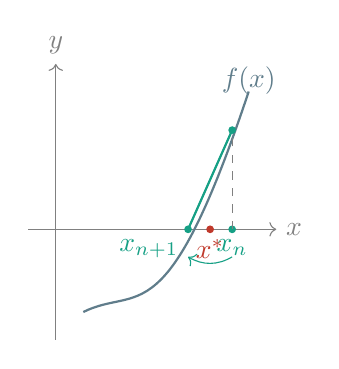
\begin{tikzpicture}[scale=0.7]
        \draw[->, gray] (-0.5,0) -- (4,0) node[right] {$x$};
        \draw[->, gray] (0,-2) -- (0,3) node[above] {$y$};
        
        % 函数曲线
        \draw[thick, headerblue] (0.5,-1.5) .. controls (1.5, -1) and (2, -2) .. (3.5, 2.5);
        \node[headerblue] at (3.5, 2.7) {$f(x)$};
        
        % 根
        \fill[accentcolor] (2.8, 0) circle (2pt) node[below] {$x^*$};
        
        % x_n
        \def\xn{3.2}
        \def\fxn{1.8} % 假装的 f(xn)
        \fill[section2] (\xn, 0) circle (2pt) node[below] {$x_n$};
        \draw[dashed, gray] (\xn, 0) -- (\xn, \fxn);
        \fill[section2] (\xn, \fxn) circle (2pt);
        
        % 切线
        \draw[thick, section2] (\xn, \fxn) -- (2.4, 0); % 切线交于 x_{n+1}
        \fill[section2] (2.4, 0) circle (2pt) node[below left] {$x_{n+1}$};
        
        % 箭头
        \draw[->, section2, bend left] (\xn, -0.5) to (2.4, -0.5);
    \end{tikzpicture}
    \end{center}

    \hspace{1em}数值分析是数学与计算机妥协的产物。我们放弃了“解析解”的完美,换取了“数值解”的通用与高效。
    \vspace{4pt}
    
    \subt{三大核心视角}
    \begin{itemize}[itemsep=4pt]
        \item \textbf{迭代即逼近}: 
        既然无法一步登天,那就步步为营。只要误差在缩小,我们终将到达真理的彼岸 (或足够近的地方)。
        
        \item \textbf{离散即近似}: 
        微分变成差分,积分变成求和。微积分的极限定义在计算机里变成了微小的 $\Delta x$。
        
        \item \textbf{条件即命运}: 
        如果问题本身是病态的 (条件数大),再好的算法也救不了。输入的一点点噪音,会导致输出面目全非。
    \end{itemize}
    
    \vspace{6pt}
    \centering\textit{\footnotesize 所有的计算都是近似,问题在于你允许多少误差。}
\end{mybox}

\end{multicols*}

\end{document}
